% !TeX spellcheck = en_US
\documentclass[aspectratio=1610]{beamer}
\usetheme{Madrid}
\setbeamercovered{transparent}
\setbeamertemplate{navigation symbols}{}
\setbeamertemplate{itemize items}[circle]
\setbeamertemplate{enumerate items}[default]

\makeatletter
\define@key{beamerframe}{wide}[10pt]{%
	\def\beamer@cramped{\itemsep #1\topsep0.5pt\relax}}
\makeatother
	

\usepackage[english]{babel}
\usepackage[utf8]{inputenc}
\usepackage[T1]{fontenc}
\usepackage{array}
\usepackage{xcolor}
\usepackage{colortbl}
\usepackage{booktabs}

\title[Winter - Lecture 10] % (optional, use only with long paper titles)
{Intermediate Macroeconomics: Lecture  W10 (Ch.15 and 18)}
\subtitle{ECON 311 -- Intermediate Macroeconomics}

\author{Muhebullah Karimzada}
\institute{School of Economics \\\ University of Northern British Columbia}
\date{Fall 2026}


% ---------- UNBC COLORS ----------
\usepackage{xcolor}
\definecolor{UNBCGreen}{RGB}{0,102,51}
\definecolor{UNBCDark}{RGB}{0,74,37}
\definecolor{UNBCGold}{RGB}{189,155,96}
\definecolor{SoftCream}{RGB}{249,247,242}
\definecolor{SoftGray}{RGB}{244,246,248}
\definecolor{AccentBlue}{RGB}{41,98,255}
\definecolor{AccentOrange}{RGB}{230,126,34}
\definecolor{AccentTeal}{RGB}{0,150,136}
\definecolor{AccentRed}{RGB}{192,57,43}
\setbeamercolor{normal text}{fg=black,bg=white}
\setbeamercolor{structure}{fg=UNBCDark}
\setbeamercolor{title}{fg=white,bg=UNBCDark}
\setbeamercolor{subtitle}{fg=UNBCGold}
\setbeamercolor{frametitle}{fg=white,bg=UNBCDark}
\setbeamercolor{block title}{fg=white,bg=UNBCDark}
\setbeamercolor{block body}{fg=black,bg=SoftGray}
\setbeamercolor{block title alerted}{fg=white,bg=AccentRed}
\setbeamercolor{block body alerted}{fg=black,bg=SoftGray}
\setbeamercolor{item}{fg=UNBCDark}
\setbeamercolor{section in toc}{fg=UNBCDark}
\setbeamercolor{alerted text}{fg=AccentRed}
\setbeamercolor{author in head/foot}{fg=white,bg=UNBCDark}
\setbeamercolor{date in head/foot}{fg=white,bg=UNBCDark}
% ---------- UNBC BRANDING ----------
\usepackage{graphicx}
\usepackage{lmodern}
\usepackage{tcolorbox}
\usepackage{tikz}
\usetikzlibrary{positioning,calc}
\setbeamertemplate{headline}{}
\setbeamertemplate{footline}{%
  \leavevmode%
  \hbox{%
  \begin{beamercolorbox}[wd=.78\paperwidth,ht=2.8ex,dp=1.2ex,leftskip=1em]{author in head/foot}%
  \color{white}\textbf{ECON 311} \hspace{0.5em} \textcolor{UNBCGold}{|} \hspace{0.5em} Intermediate Macroeconomics%
  \end{beamercolorbox}%
  \begin{beamercolorbox}[wd=.22\paperwidth,ht=2.8ex,dp=1.2ex,rightskip=1em plus1fil]{date in head/foot}%
  \color{white}\insertframenumber/\inserttotalframenumber%
  \end{beamercolorbox}}%
}

\newtcolorbox{mybox}[2][]{
  colback=#2!8,
  colframe=#2,
  boxrule=0.8pt,
  arc=2mm,
  left=2mm,right=2mm,top=1.5mm,bottom=1.5mm,
  #1
}

\newcommand{\topbanner}[1]{%
\begin{tikzpicture}[remember picture,overlay]
\fill[UNBCGold] ([yshift=-0.65cm]current page.north west) rectangle ([yshift=-0.48cm]current page.north east);
\node[anchor=north west,font=\small\bfseries,text=UNBCDark] at ([xshift=0.35cm,yshift=-0.78cm]current page.north west) {#1};
\end{tikzpicture}%
}
\begin{document}

\begin{frame}[plain]
  \titlepage
\end{frame}

\begin{frame}[wide]{Quantitative DSGE Models}
	\begin{itemize}
		\item Full DSGE models incorporate the complete dynamic response of all economic variables to all shocks
		\item The Smets–Wouters (2007) model is used by macroeconomic forecasters and central banks around the world as a building block 
		\begin{itemize}
			\item Incorporates shocks previously discussed 
			\item Includes both sticky prices and sticky wages and more
		\end{itemize}
		
		\item One of the key advantages of this type of model is that is can be estimated
		\begin{itemize}
			\item By “estimated,” we mean that the parameters of the DSGE model are chosen to make the model match the data for the U.S. economy as accurately as possible
		\end{itemize}
	\end{itemize}
\end{frame}

\begin{frame}[wide]{Shocks}
	\begin{itemize}
		\item Quantitative DSGE models incorporate multiple shocks simultaneously
		\item The Smets-Wouters model features:
		\begin{itemize}
			\item Productivity shocks
			\item Shocks to government purchases
			\item Financial frictions
			\item Investment shocks
			\item Labour market shocks
			\item Shocks to markups in product markets
		\end{itemize}
		
	\end{itemize}
\end{frame}

\begin{frame}[wide]{Impulse Response Functions}
	\begin{itemize}
		\item Impulse Response Functions (IRF) is one of the main tool to analyze the DSGE model (and multivariate time series model)
		\item The IRF shows how one macroeconomic variable of interest responds over time to an economic shock
		\item Each graph shows how each variables responses to a temporary shock
		\item The next slide shows the IRF for GDP in the estimated Smets-Wouters model
		\begin{itemize}
			\item By what percent does GDP change after a temporary 1 percentage point increase in the fed funds rate?
		\end{itemize}
	\end{itemize}
\end{frame}



\begin{frame}[wide]{The Response of GDP to a Monetary Policy Shock}
	\begin{itemize}
		\item A 1 \% increase in the fed funds rate causes GDP to fall by about 0.2 \% in the first quarter after the shock
		\item At its peak three to four quarters after the shock, GDP is lower by 0.33 \%
	\end{itemize}
	\begin{figure}
		\centering
		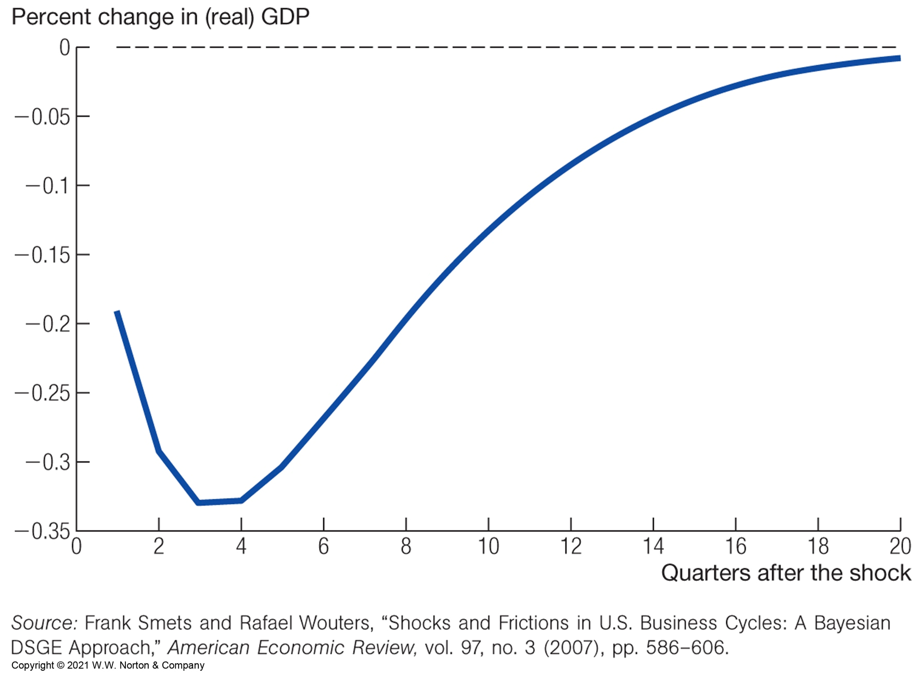
\includegraphics[width=0.55\linewidth]{Figures/fig_15_01}
	\end{figure}
	
\end{frame}


\begin{frame}[wide]{The Dynamic Effects of a Monetary Policy Shock}
	\begin{itemize}
		\item The DSGE models include many other variables, like consumption, hours worked, and inflation, allow us to study how each of these variables responds to a shock
		\item The response of the economy looks very much like the response we saw in our AS/AD framework 
	\end{itemize}
	\begin{figure}
		\centering
		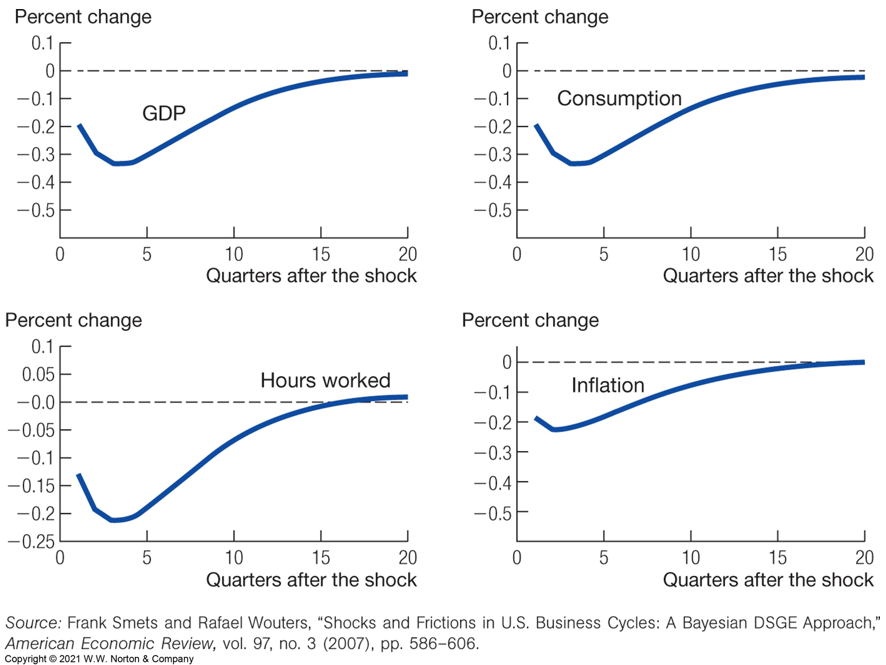
\includegraphics[width=0.5\linewidth]{Figures/fig_15_02}
	\end{figure}
	
\end{frame}

\begin{frame}[wide]{The Dynamic Effects of a Monetary Policy Shock}
	\begin{itemize}
		\item When there is a surprise tightening of monetary policy (a rise in interest rate), there are less investment
		\item As a result, less output to be produced which lower the consumption 
		\begin{itemize}
			\item Given the permanent income hypothesis, the consumption should varies less than the output
			\item But Smets-Wouters's  substantial adjustment costs to investment causes consumption to move by more (if the output is not being used in investment, it would go toward consumption)
			\item Yet, a good model should not imply that the consumption move more than output
		\end{itemize}
		\item As the output fall, according to the PC, the inflation rate should fall
	\end{itemize}
\end{frame}

\begin{frame}[wide]{The Dynamic Effects of a TFP Shock}
	\begin{figure}
		\centering
		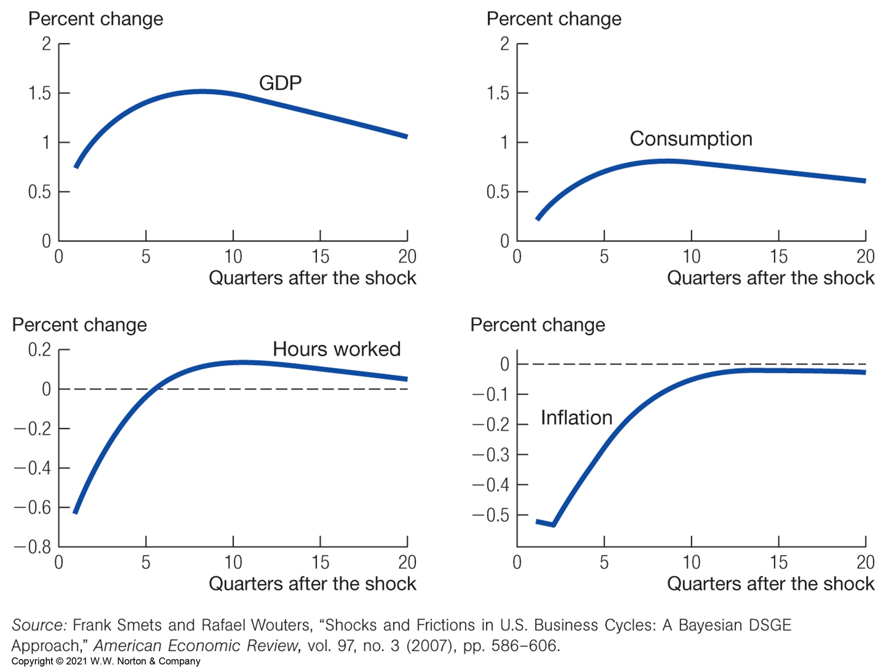
\includegraphics[width=0.6\linewidth]{Figures/fig_15_03}
	\end{figure}
\end{frame}

\begin{frame}[wide]{The Dynamic Effects of a TFP Shock}
	\begin{itemize}
		\item The TFP shocks considered here decade over time instead of disappear entirely in one period
		\item As the positive TFP shocks arrive, the GDP rises
		\begin{itemize}
			\item The increase is even higher than the the increase in the TFP (i.e., 1\%)
			\item This is because of the capital accumulation, which is similar to the case discussed in the Solow model
		\end{itemize}
		\item Given the permanent income hypothesis, individual prefer to smooth consumption.
		\begin{itemize}
			\item The consumption increases less than the increase in output
		\end{itemize}
	\end{itemize}
\end{frame}

\begin{frame}[wide]{The Dynamic Effects of a TFP Shock}
	\begin{itemize}
		\item The hour worked may look puzzling, as the stylized model would suggest an increase in both wage and employment
		\begin{itemize}
			\item This model feature sticky prices, the firm supply as many as amount demanded
			\item Since the consumption rises by little, the rise in TFP is more than enough to supply the mount demanded in the economy
		\end{itemize}
		\item The TFP shocks also raises potential GDP and expands supply in the economy
		\begin{itemize}
			\item In the AS/AD model, this shifts down the AS curve 
			\item However, the actual output doesn't increase as much as the shock initially, the actual output would be lower than the potential output temporary 
			\item Resulting a fall in inflation rate
		\end{itemize}
	\end{itemize}
\end{frame}

\begin{frame}[wide]{The Dynamic Effects of a Shock to Government Purchases}
	\begin{figure}
		\centering
		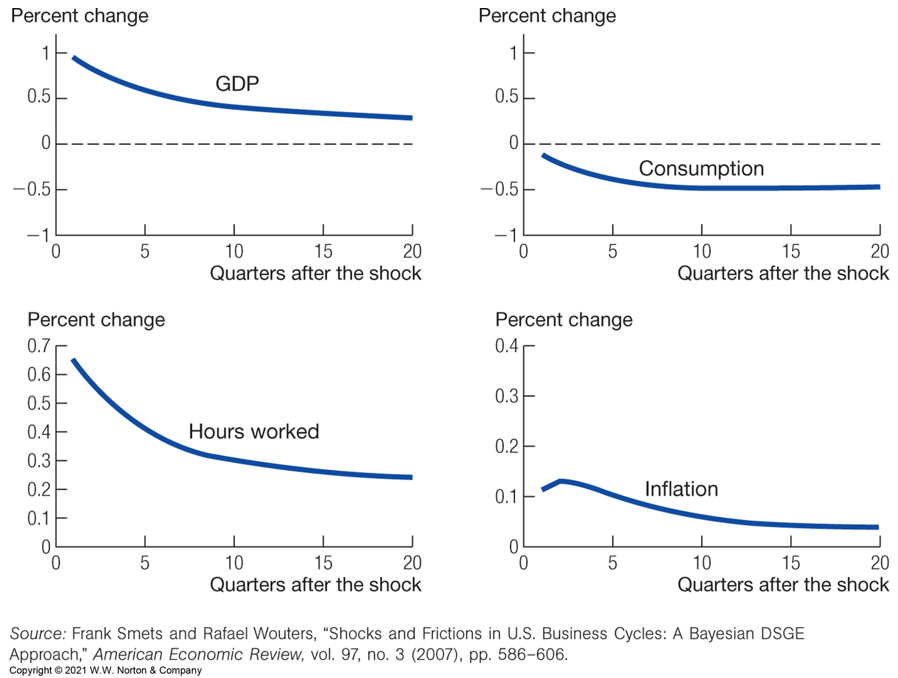
\includegraphics[width=0.6\linewidth]{Figures/fig_15_04}
	\end{figure}
	
\end{frame}

\begin{frame}[wide]{The Dynamic Effects of a Shock to Government Purchases}
	\begin{itemize}
		\item The stylized model suggests that the wages would fall while the hours worked increases
		\begin{itemize}
			\item As the government increases its spending, consumer would expect an increase in tax at some point
			\item The wealth decrease and lead to a decrease in consumption
			\item The labour supply shift to the right 
		\end{itemize}
		\item The model generate similar response as expected
		\item Since the labour supply increases, the effect on inflation is little
	\end{itemize}
\end{frame}

\begin{frame}[wide]{The Dynamic Effects of a Financial Frictions Shock}
	\begin{figure}
		\centering
		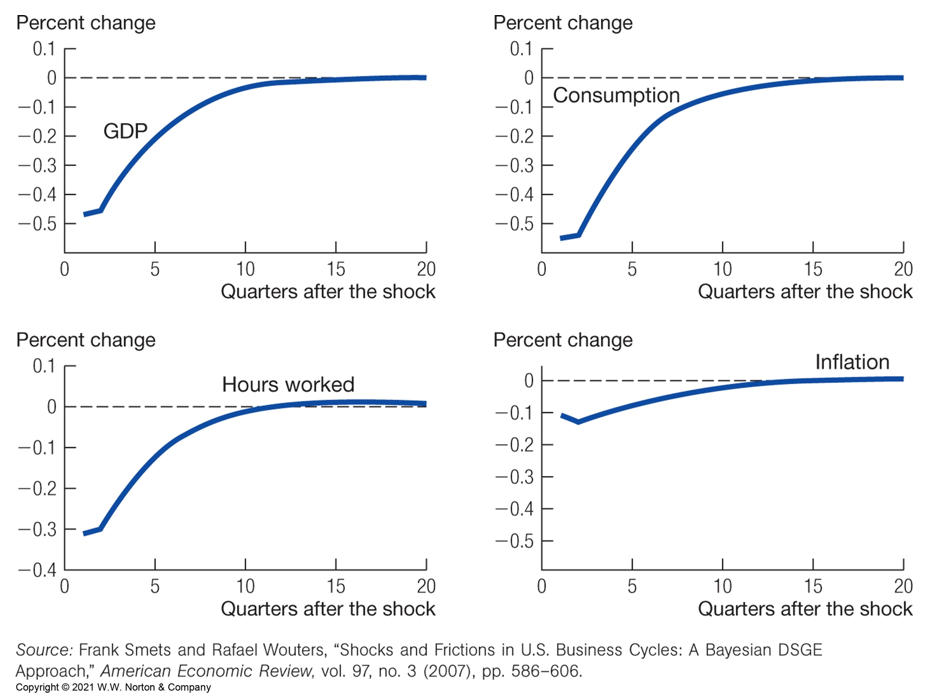
\includegraphics[width=0.6\linewidth]{Figures/fig_15_05}
	\end{figure}
\end{frame}

\begin{frame}[wide]{The Dynamic Effects of a Financial Frictions Shock}
	\begin{itemize}
		\item This particular financial shock implemented as a wedge between the rate of saving and borrowing, because of asymmetric information problem
		\begin{itemize}
			\item Implies it has the largest effect on consumption
		\end{itemize}
		\item Otherwise, the shock looks very similar to a monetary policy shock, as both work through interest rates
	\end{itemize}
\end{frame}

\begin{frame}[wide]{Conclusion}
	\begin{itemize}
		\item Macroeconomists argue about the importance of various shocks and various frictions in accounting for economic fluctuations
		\begin{itemize}
			\item These arguments often center around the extent to which certain frictions are quantitatively important
			\begin{itemize}
				\item How sticky are wages and prices?
				\item How important are credit market frictions?
				\item How elastic is labor supply in the economy?
			\end{itemize}
		\end{itemize}
	\end{itemize}
\end{frame}

\begin{frame}[wide]{Conclusion}
	\begin{itemize}
		\item The basic framework we should use to understand macroeconomic fluctuations developed over the past 50 years
		\begin{itemize}
			\item A key element is a basic growth model like the Solow model
			\item Including more microfoundation elements
		\end{itemize}
		\item The basic DSGE framework has been enriched in many ways recently
		\item The models make precise quantitative predictions about the complete dynamics of a host of endogenous variables
	\end{itemize}
\end{frame}

\begin{frame}[wide]{What are You Going to Learn (Ch. 18)}
	\begin{itemize}
		\item Government spending, taxation, budget deficits, and the debt-GDP ratio nationally and globally
		\item The government’s intertemporal budget constraint
		\item The economic consequences of budget deficits
		\item The fiscal problem of the twenty-first century: how to finance rising health expenditures
	\end{itemize}
\end{frame}

\begin{frame}[wide]{Introduction}
	\begin{itemize}
		\item The government can finance expenditures by
		\begin{itemize}
			\item using tax revenue
			\item printing money
			\item borrowing
		\end{itemize}
		\item But the government’s budget must balance in present value
		\begin{itemize}
			\item The amount the government spends must equal the amount the government earns in terms of present value
			\item Budget deficits today must be offset by budget surpluses in the future
		\end{itemize}
		\item The “fiscal problem of the twenty-first century” 
		\begin{itemize}
			\item If current policies remain unchanged, forecasts show the U.S. and many other countries' deficits and debt-to-GDP ratios will explode
		\end{itemize}
		
	\end{itemize}
\end{frame}

\begin{frame}[wide]{U.S. Government Spending and Revenue}
	\begin{itemize}
		\item In 2018, government spending in the United States was 
		\begin{itemize}
			\item \$6.7 trillion
			\item 20.0 percent of GDP
			\item more than \$20,500 per person
		\end{itemize}
		\item Tax revenues were 16.2 percent of GDP 
	\end{itemize}
\end{frame}

\begin{frame}[wide]{The U.S. Federal Government Budget, 2018}

	\begin{figure}
		\centering
		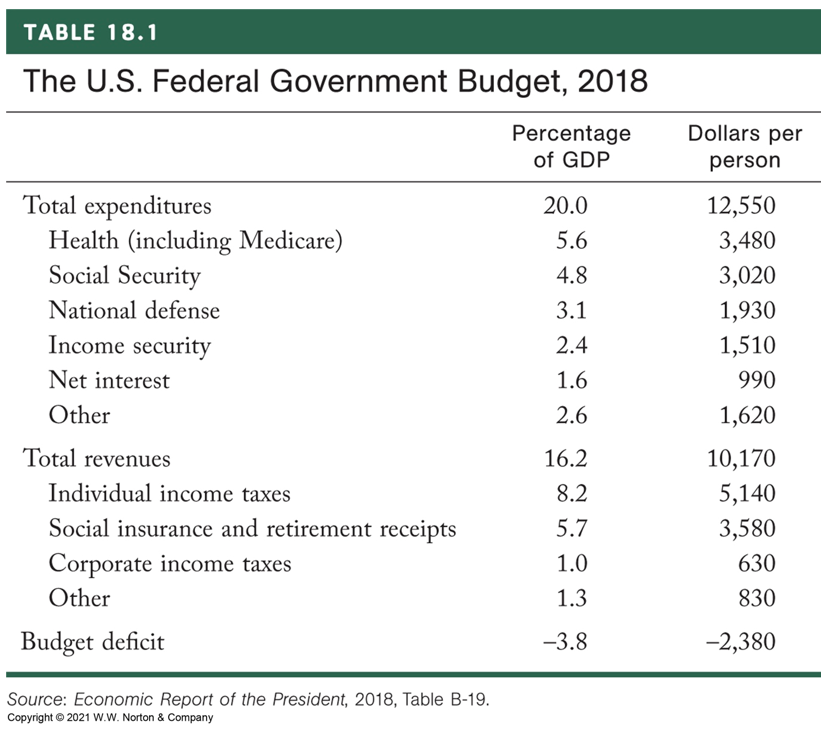
\includegraphics[width=0.5\linewidth]{Figures/fig_16_01}
	\end{figure}
	
\end{frame}

\begin{frame}[wide]{The U.S. Federal Government Budget, 2018}
	\begin{itemize}
		\item It is expected that the expenditure healthcare as a fraction of GDP will increase over time, because:
		\begin{itemize}
			\item Federal entitlements are becoming more generous
			\item A growing proportion of the population qualifies for benefits
			\item With rising income, expenditure on healthcare is expected to increase at a faster rate than consumption
		\end{itemize}
	\end{itemize}	
\end{frame}

\begin{frame}[wide]{Government Spending and Revenue}
	\begin{itemize}
		\item The budget balance: The difference between tax revenues and spending
		\item A budget surplus: Tax revenues > Spending
		\item A budget deficit:	Tax revenues < Spending
		\begin{itemize}
			\item The government must borrow by selling bonds
		\end{itemize}
		\item A balanced budget: Tax revenues = Spending
	\end{itemize}
\end{frame}

\begin{frame}[wide]{Government Spending and Revenue}
	\begin{itemize}
		\item In 2018, there was a budget deficit equal to 3.8 percent of GDP
		\begin{itemize}
			\item The government does not usually sell assets to finance the deficit
			\item Usually, the government borrows from lenders within the United States and abroad
		\end{itemize}
		\item When the government sells bonds, they use the money as a loan
		\begin{itemize}
			\item Suppose a 10-year bond issued in 2021 pays \$100 when it matures in 2031
			\item In 2021, the investor may pay \$55 for this bond (and that amount is the loan to the government)
			\item The remaining \$45 the government pays is the nominal interest
		\end{itemize}
		\item In 2018, the government issued more than \$750 billion in new bonds (>\$2,300 per person)
	\end{itemize}
\end{frame}


\begin{frame}[wide]{Spending and Revenue over Time}
	\begin{itemize}
		\item After World War II, spending and tax revenues rose to about 18 percent of GDP
		\begin{itemize}
			\item The two were roughly the same fraction of the GDP
		\end{itemize}
		\item In 1970, systematic budget deficits began to emerge
		\begin{itemize}
			\item Deficits as a fraction of GDP peaked in 1983
			\item There was a brief surplus in 1998, followed by another deficit in 2002
		\end{itemize}
		\item In 2009, the budget deficit was around 10 percent of GDP
		\begin{itemize}
			\item During the recession, tax revenues fell and government spending increased
		\end{itemize}
	\end{itemize}
\end{frame}

\begin{frame}[wide]{U.S. Federal Government Revenue and Spending}
	\begin{figure}
		\centering
		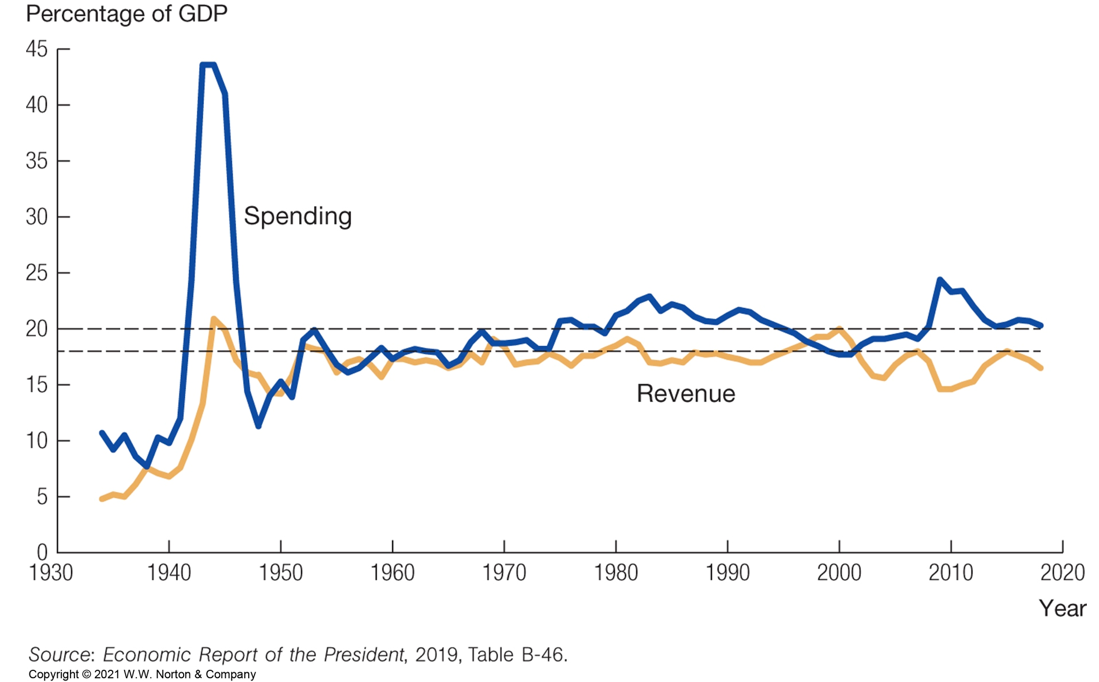
\includegraphics[width=0.7\linewidth]{Figures/fig_16_02}
	\end{figure}
	
\end{frame}

\begin{frame}[wide]{The Debt-GDP Ratio}
	\begin{itemize}
		\item Government debt: outstanding stock of bonds that have been issued in the past
		\item In 2005, the debt-GDP ratio was just over 35 percent
		\item In 2018, the debt-GDP ratio was nearly 80 percent, a huge increase
		\item About half of the debt in recent years is owed to foreigners
	\end{itemize}
\end{frame}

\begin{frame}[wide]{The Debt-GDP Ratio}
	\begin{itemize}
		\item The government itself also holds a large amount of bonds
		\begin{itemize}
			\item The Social Security trust fund that will be paid to future retirees held \$2.7 trillion in assets in 2014
			\item One branch of government loaning to another has no affect on government “wealth.”
			\begin{itemize}
				\item The asset and debt created offset one another
			\end{itemize}
		\end{itemize}
	\end{itemize}
\end{frame}

\begin{frame}[wide]{Federal Debt and Deficits in the United States}
	\begin{figure}
		\centering
		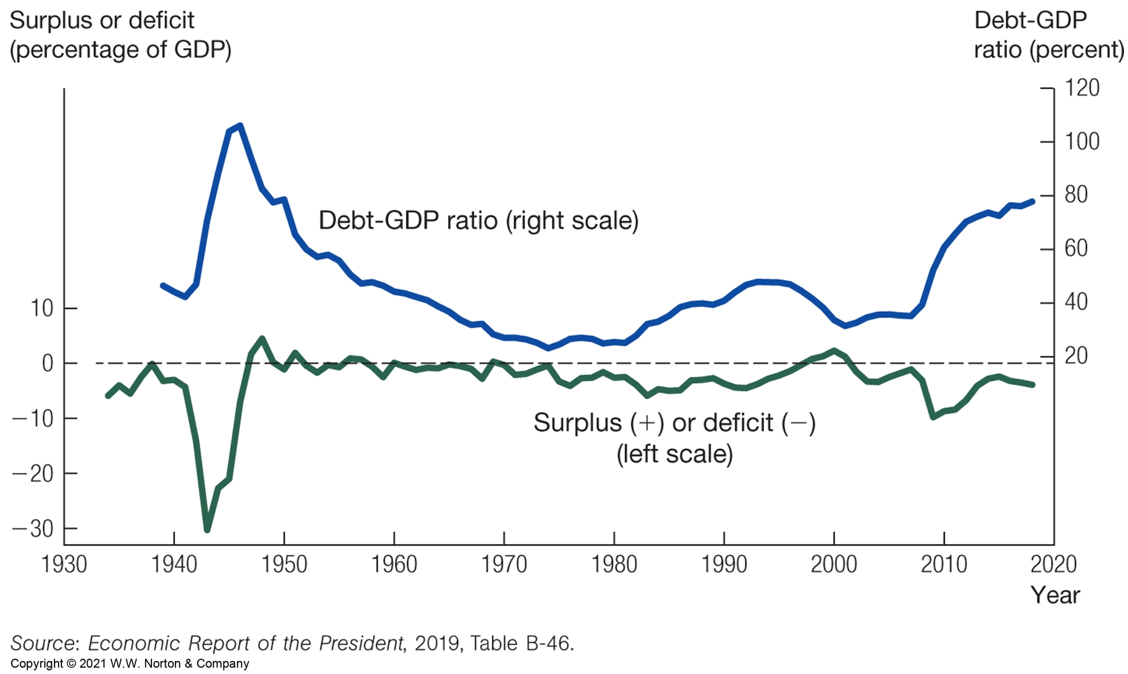
\includegraphics[width=0.7\linewidth]{Figures/fig_16_03}
	\end{figure}
\end{frame}

\begin{frame}[wide]{International Evidence on Spending and Debt}
	\begin{itemize}
		\item Among the richer OECD countries, the United States has a lower than average
		\begin{itemize}
			\item government spending-to-GDP ratio
			\item debt-GDP ratio
		\end{itemize}
		\item Norway is an exception among many rich countries
		\begin{itemize}
			\item Negative debt-GDP ratio
			\item Norway benefits from large government-owned petroleum and natural gas reserves, which boost its revenues and lead to budget surpluses
			\item Knowing these revenues will be depleted, the Norwegian government saves these surpluses as assets in a Government Petroleum Fund to finance future government spending
		\end{itemize}
		
	\end{itemize}
\end{frame}

\begin{frame}[wide]{Government Spending around the World, 2017}
	\begin{figure}
		\centering
		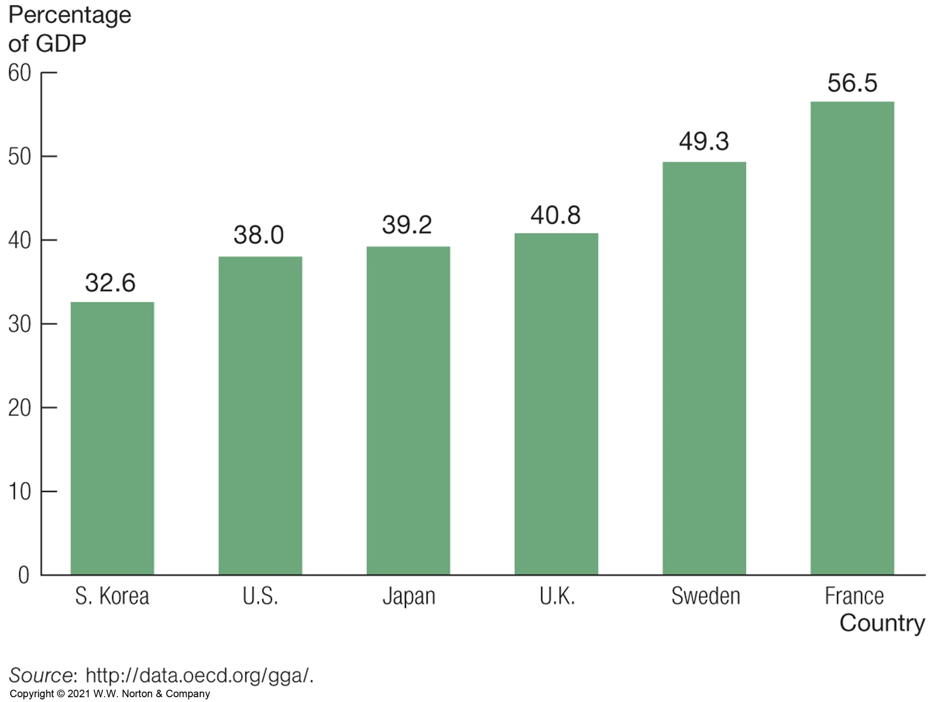
\includegraphics[width=0.7\linewidth]{Figures/fig_16_04}
	\end{figure}
\end{frame}

\begin{frame}[wide]{Debt-GDP Ratios around the World}
	\begin{itemize}
		\item In Japan, the ratio has risen sharply since 1995, from a low of about 20 percent to a high of more than 120 percent in 2018
	\end{itemize}
	\begin{figure}
		\centering
		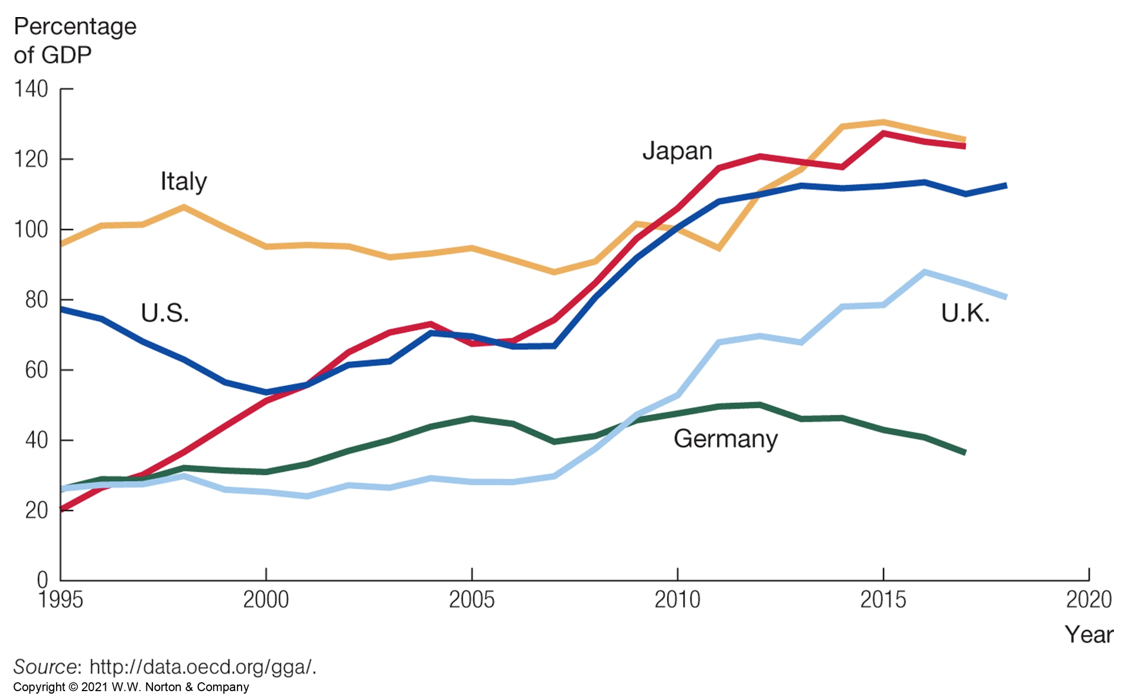
\includegraphics[width=0.6\linewidth]{Figures/fig_16_05}
	\end{figure}
\end{frame}

\begin{frame}[wide]{Debt-GDP Ratios around the World}
	\begin{itemize}
		\item The net debt to GDP ratio varies a lot across country. But, higher number does not always mean a country is at risk. It depends on many country specific factor
	\end{itemize}
	\begin{figure}
		\centering
		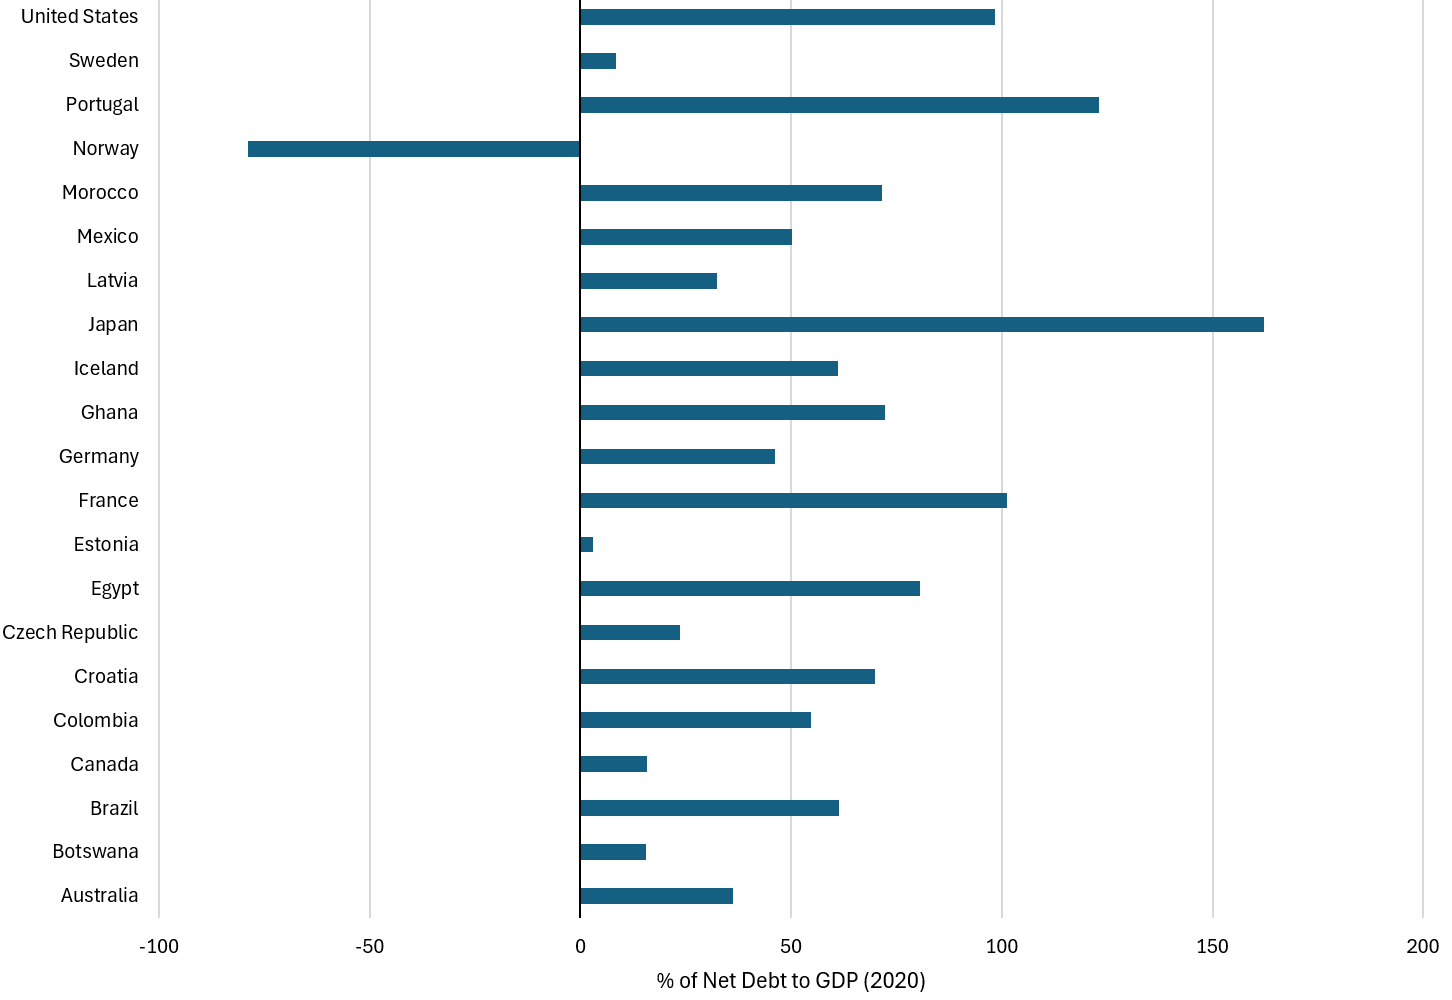
\includegraphics[width=0.7\linewidth]{Figures/fig_16_06}
	\end{figure}
	
\end{frame}

\begin{frame}[wide]{Debt-GDP Ratios around the World}
	\begin{itemize}
		\item The Debt-GDP ratio comprises two components: Debt and GDP
		\item If the GDP kept growing faster than debt, the debt-GDP ratio could decrease
		\item When assessing the risk of a country defaulting, it's necessary to project the future growth of the country
		\begin{itemize}
			\item Many factor could come into place as we learn in previous chapter
		\end{itemize}
	\end{itemize}

\end{frame}

\begin{frame}[wide]{The Government Budget Constraint}
	\begin{itemize}
		\item The flow version of the government budget constraint holds in each period
		\item The sources of funds to the government must equal the uses of funds
		\[G_t + Tr_t + iB_t = T_t + \Delta B_{t+1} + \Delta M_{t+1}\]
		\item[] where $G_t$ is the gov't purchases, $Tr_t$ is the transfer payment, $iB_t$ is the interest payments on debts, $T_t$ is the taxes, $\Delta B_{t+1}$ is the New Borrowing and $\Delta M_{t+1}$ is the change in money stock
		\item $\Delta B_{t+1}$ and $\Delta M_{t+1}$ can be negative
	\end{itemize}
\end{frame}

\begin{frame}[wide]{The Government Budget Constraint}
	\begin{itemize}
		\item Assume for this chapter
		\begin{itemize}
			\item The change in the stock of money is zero ($\Delta M_{t+1}$)
			\item Transfer payments are zero ($Tr_t = 0$)
		\end{itemize}
		\[B_{t+1} = (1+i) B_t + G_t -T_t\]
		\item LHS is the stock of debt at the start of next year 
		\item RHS is the Stock of debt this year, including the required interest payments plus the budget deficit
		\item The primary deficit: $G_t - T_t$
		\begin{itemize}
			\item If the $G_t-T_t=0$, then the growth of $B$ is $g_B = \frac{B_{t+1}}{B_t} - 1 = i$
		\end{itemize}
		\item The total deficit: $G_t +iB_t -T_t$		
	\end{itemize}
\end{frame}

%\begin{frame}[wide]{The Intertemporal Budget Constraint}
%	\begin{itemize}
%		\item 
%	\end{itemize}
%\end{frame}
%
%\begin{frame}[wide]{The Intertemporal Budget Constraint}
%	\begin{itemize}
%		\item 
%	\end{itemize}
%\end{frame}
%
%\begin{frame}[wide]{The Intertemporal Budget Constraint}
%	\begin{itemize}
%		\item 
%	\end{itemize}
%\end{frame}

%\begin{frame}[wide]{An Increase in the Investment Rate}
%	\begin{columns} 
%			% Column 1
%			\begin{column}{.5\textwidth}
%				\begin{itemize}
%					\item Suppose the investment rate increases permanently for exogenous reasons ($s'>s$)
%					\begin{itemize}
%						\item The investment curve rotates upward ($\bar{s}'\bar{A}  \bar{L}^{1-\alpha} K_t^\alpha > \bar{s}\bar{A}  \bar{L}^{1-\alpha} K_t^\alpha$)
%						\item The depreciation curve remains unchanged ($\delta K_t$)
%						\item The capital stock increases by transition dynamics to reach the new steady state
%						\begin{itemize}
%							\item This happens because investment exceeds depreciation ($sY_t>\delta K_t$)
%						\end{itemize}
%						\item The new steady state is located to the right
%					\end{itemize}
%				\end{itemize}
%			\end{column}
%			% Column 2    
%			\begin{column}{.5\textwidth}			
%				\begin{figure}
%					\centering
%					\includegraphics[width=1\linewidth]{"Figures/An Increase in the Investment Rate"}
%				\end{figure}
%			\end{column}%
%		\end{columns}
%\end{frame}

%\begin{frame}[wide]{Measuring the State of the Economy}
%	\begin{columns} 
%		% Column 1
%		\begin{column}{.5\textwidth}
%			\begin{table}[htbp]
%				\centering
%				\begin{tabular}{lrrrr}
%					& 2005  & 2006  & 2007  & 2008 \\
%					\hline
%					GDP   & 12.6  & 13.4  & 14.0    & 14.3 \\
%					(in trillions of \$) &       &       &       &  \\
%					Growth rate GDP &       & 0.063 & 0.045 & 0.021 \\
%					\hline
%				\end{tabular}%
%				\label{tab:addlabel}%
%			\end{table}%
%		\end{column}
%		% Column 2    
%		\begin{column}{.5\textwidth}			
%			
%			
%		\end{column}%
%	\end{columns}
%\end{frame}

\begin{frame}[wide]{Next Lecture}
	\begin{itemize}
		\item Next lecture will finish Ch.18
	\end{itemize}
\end{frame}

\end{document}